% Chapter Template

\chapter{Results} % Main chapter title
\label{chap:results}
%B-Feld. Von welchem Instrument? auch RTN-System. Genauso Winkel berechnet.
%1-min-Mittel (Gyroradius Zeit zeigen) und entsprechend EpQ-Steps den PHAs zugeordnet.
%
%
%
Here we present first results of the method that has been developed in chapter \ref{chapter:data} for $\mathrm{He^{+}}$. For creating three-dimensional velocity spectra from $\mathrm{He^{+}}$ SWICS PHA data we synchronize the selected data (s. \ref{chapter:instrumentation}, $\mathrm{He^{+}}$ Triple Coincidences) with the spacecraft's aspect angle, its eigen-velocity and the present solar wind speed.
This gives us directionally resolved counts from the observed phase space volume.
\\ \\
An example for data of a measuring period of 50 days in 1993, limited to solar wind speeds from $760 \, \mathrm{km\,s^{-1}}$ to $780 \, \mathrm{km\,s^{-1}}$, is shown in Fig. \ref{fig:counts_50}. Here we histogrammed the counts by utilizing Cartesian $w_{\mathrm{sw,R}}$, $w_\mathrm{sw,T}$ and $w_\mathrm{sw,N}$ bins in solar wind frame. Shown are counts from a ``slice'' in the $w_\mathrm{sw,T} - w_\mathrm{sw,N}$ plane. Counts within the range $0.3 <= w_\mathrm{sw,R} < 0.5$ have been summarized for each $w_\mathrm{sw,T} - w_\mathrm{sw,N}$ bin. The orientation of this cut is sketched in Fig. \ref{fig:sketch_slice_R} for better understanding.\\
\begin{figure}[h]
	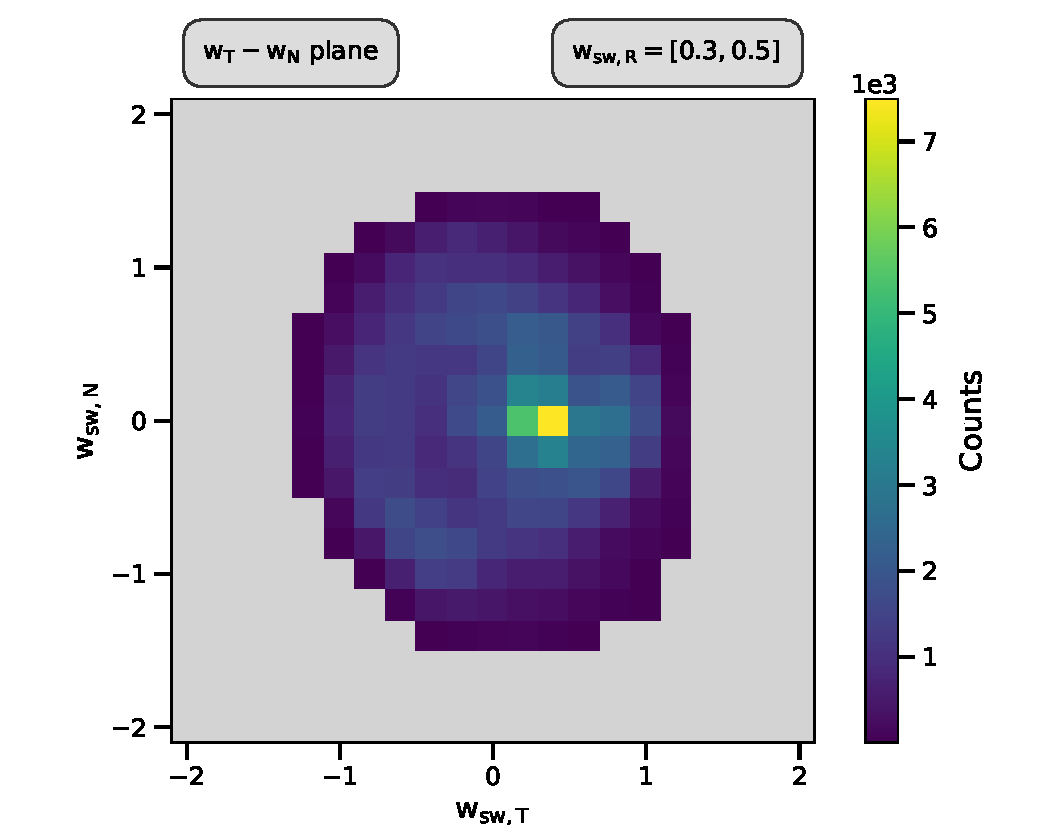
\includegraphics[width=.85\textwidth]{Figures/slice_50_counts.pdf}
	\centering
	\caption{Cartesian cut through $\mathrm{He^{+}}$ count distribution in a 3D $w_\mathrm{sw}$-space, measured during DOY 315-365 in 1993 for solar wind speeds from $760 \, \mathrm{km\,s^{-1}}$ to $780 \, \mathrm{km\,s^{-1}}$.}
	\label{fig:counts_50}
\end{figure}
\begin{figure}[h]
	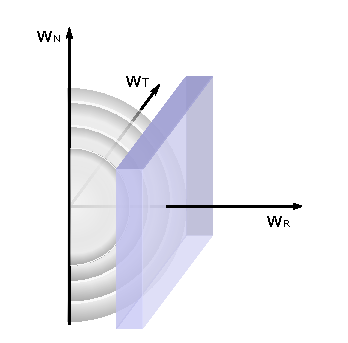
\includegraphics[width=.5\textwidth]{Figures/sketch_slice_R2.pdf}
	\centering
	\caption{Sketch of the orientation of a slice in the $w_T - w_N$ plane. A selection of ESA shells is shown in grey.}
	\label{fig:sketch_slice_R}
\end{figure}
By dividing these counts by the integrated phase space volume (PSV) for the observed time, which is binned in the same way and shown in Fig. \ref{fig:norm_50}, we yield the resulting phase space density (PSD), s. Fig. \ref{fig:psd_50}. When comparing the three Figures \ref{fig:counts_50}, \ref{fig:norm_50} and \ref{fig:psd_50} one can see a clear difference in overall shape between PSV and PSD (resp. counts). The nonzero part of the PSD does not cover all of the scanned PSV. This means that SWICS did not observe $\mathrm{He^{+}}$ PUI over all of the observed PSV but only in a distinct partial volume.\\ 
However, the 2D projection of the PSD has a roundish shape. In fact we even find a spherical shape in 3D. As a feasible visualization a stepwise sequence of $w_\mathrm{sw,T} - w_\mathrm{sw,N}$ ``slices'' is displayed in the appendix \ref{Appendix}. Each slice is again a projection of the PSD from a width $\Delta w_\mathrm{sw,R} = 0.2$. The sequence starts with $w_\mathrm{sw,R}$-values below solar wind speed with the slice $-0.5 <= w_\mathrm{sw,R} < -0.3$ and steps seamlessly up to $1.1 <= w_\mathrm{sw,R} < 1.3$ in nine increments. The radius of the projection increases slightly towards $ w_\mathrm{sw,R} \approx 0$ and then starts decreasing again for larger $w_\mathrm{sw,R}$. This suggests the three-dimensional shape of a sphere centered around $w_\mathrm{sw,R} = 0$, which is a finding that confirms the theory of an isotopic and cooled PUI VDF (s. Sec. \ref{sec:theo_vdf}). \\
For $w_\mathrm{sw,R} < 0$ and towards smaller values of $w_\mathrm{sw,R}$ an increasing ``hole'' in the PSD emerges from the center. This is due to the fact of a limited instrumental coverage for $\mathrm{He^{+}}$ at higher ESA steps, which is described in more detail in Sec. \ref{subsec:cov}. \\
Apart from taking slices from the $w_\mathrm{sw,T} - w_\mathrm{sw,N}$ plane along the $w_\mathrm{sw,R}$-axis we can also cut the three-dimensional distribution of the PSD along the other two axes. This is shown for the $w_\mathrm{sw,R} - w_\mathrm{sw,N}$ plane in Fig. \ref{fig:sketch_slice_T} and for the the $w_\mathrm{sw,R} - w_\mathrm{sw,T}$ plane in Fig. \ref{fig:sketch_slice_N}, each projection containing $w_\mathrm{sw,R} = 0$.
Both images confirm the underlying three-dimensional spherical distribution.
\\
Taking a look at the $w_\mathrm{sw,R}$-slice of the PSD in Fig. \ref{fig:psd_50} again, one sees a relatively sharp peak in the bins around $w_\mathrm{sw,T} = 0.4$ and $w_\mathrm{sw,N} = 0$. This means that this part of PSV has been observed more often than surrounding parts, which is due to the spacecraft having a substantial aspect angle $\varphi_{asp}$ at the end of the year 1993 (s. Fig. \ref{fig:aa}). Because the spacecraft's spin axis was tilted away from the radial direction for most of the time, this peak is shifted a little bit away from the center. The fact that this distinct part of PSV has been observed particularly often is followed by a qualitatively similar peak in counts, s. Fig. \ref{fig:counts_50}. 
As this peak is a result of the measurement and not a feature in the velocity distribution of $\mathrm{He^{+}}$, it vanishes with the normalization process. The PSD shows an increased density over a wider range around the radial direction, which tells that $\mathrm{He^{+}}$ tends to stream radial in this example from 1993.
\begin{figure}[h]
	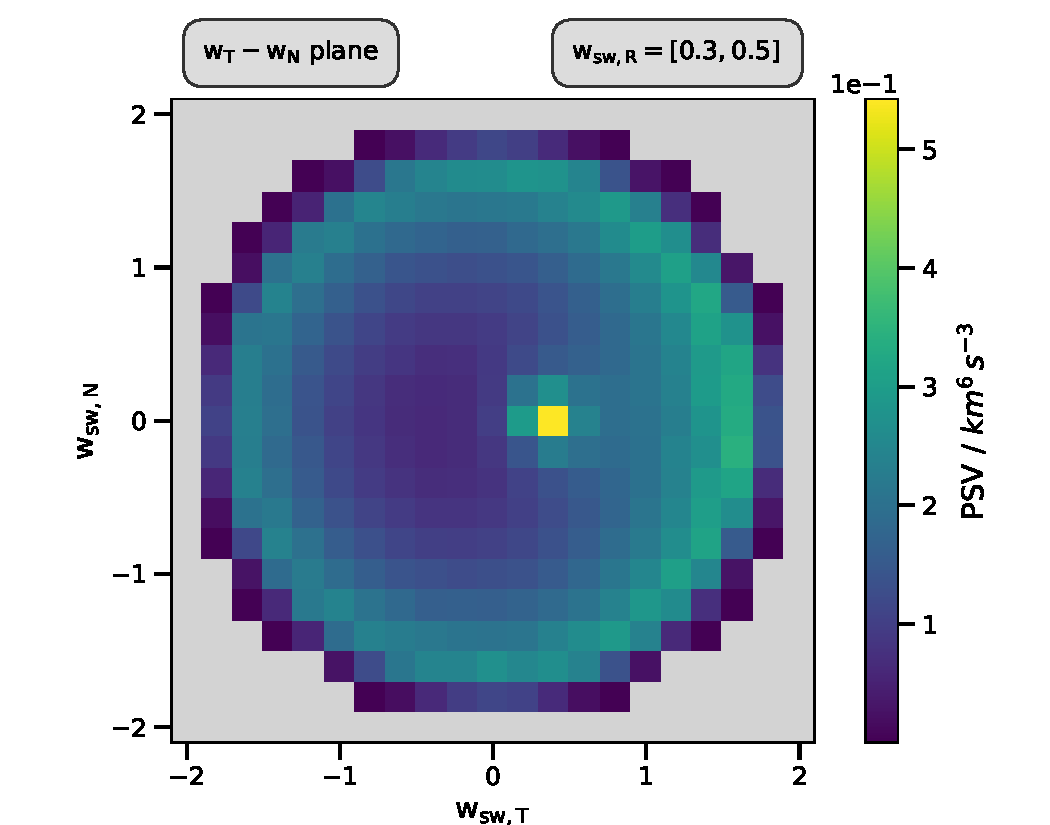
\includegraphics[width=.85\textwidth]{Figures/slice_50_norm.pdf}
	\centering
	\caption{Cartesian cut through the integrated observed PSV in a 3D $w_\mathrm{sw}$-space, measured during DOY 315-365 in 1993 for solar wind speeds from $760 \, \mathrm{km\,s^{-1}}$ to $780 \, \mathrm{km\,s^{-1}}$.}
	\label{fig:norm_50}
\end{figure}
\begin{figure}[h]
	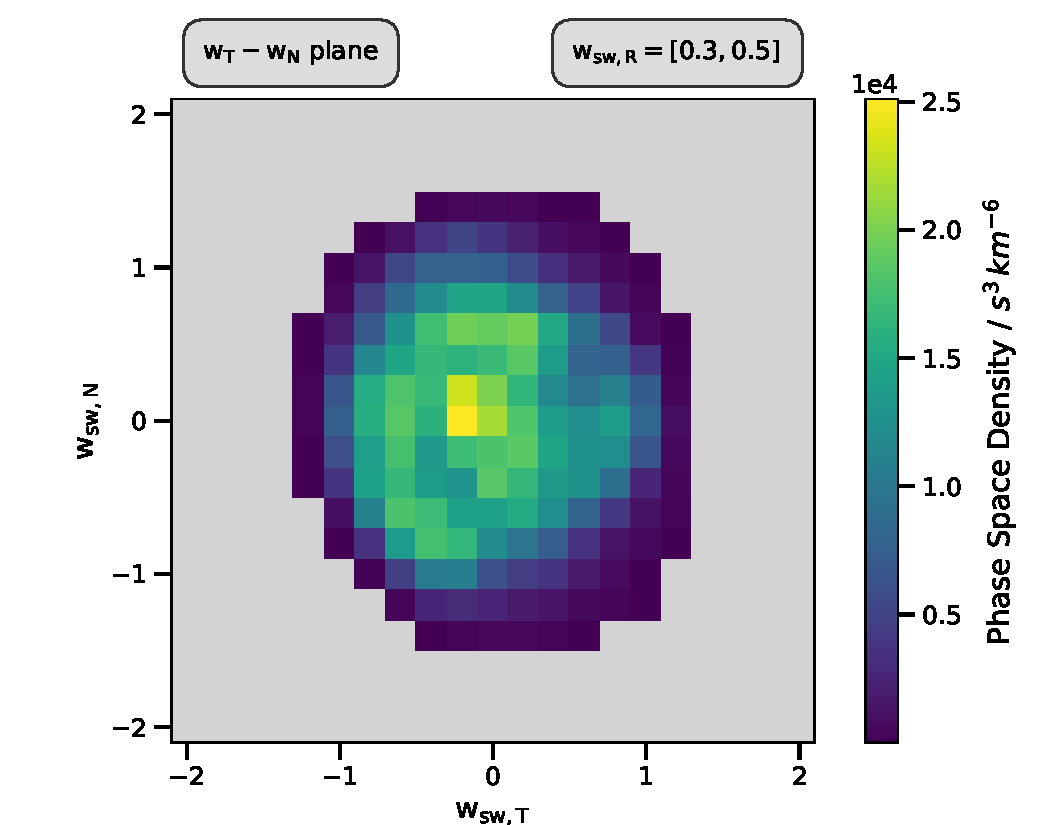
\includegraphics[width=.85\textwidth]{Figures/slices_50_3.pdf}
	\centering
	\caption{Cartesian cut through the three-dimensional PSD for $\mathrm{He^{+}}$, measured during DOY 315-365 in 1993 for solar wind speeds from $760 \, \mathrm{km\,s^{-1}}$ to $780 \, \mathrm{km\,s^{-1}}$}
	\label{fig:psd_50}
\end{figure}
% Skizzen / andere Slices:
\begin{figure}[h]
	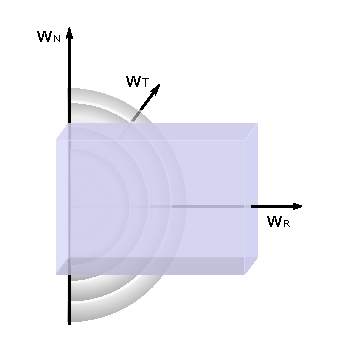
\includegraphics[width=.34\textwidth]{Figures/sketch_slice_T2.pdf}
	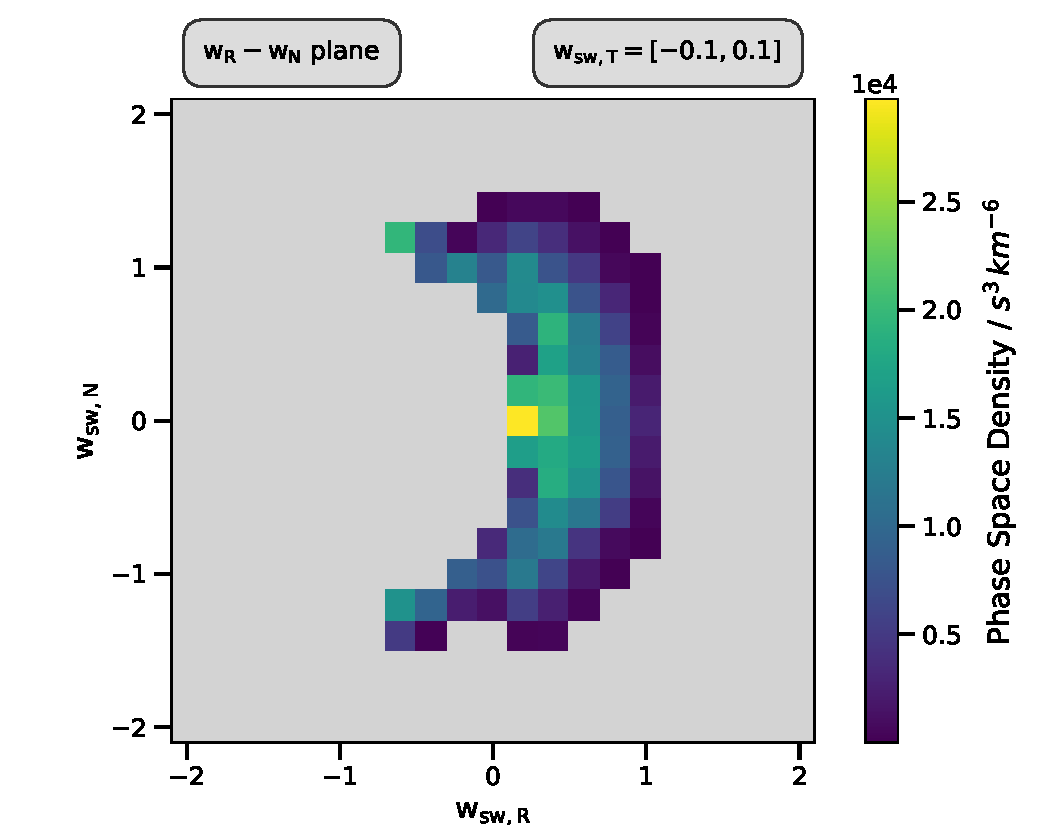
\includegraphics[width=.64\textwidth]{Figures/slice_50_T.pdf}
	\centering
	\caption{\textbf{Left:} Sketch of the orientation of a slice in the $w_R - w_N$ plane. A selection of ESA shells is shown in grey.\\ \textbf{Right:} Cartesian cut through the three-dimensional PSD for $\mathrm{He^{+}}$, measured during DOY 315-365 in 1993 for solar wind speeds from $760 \, \mathrm{km\,s^{-1}}$ to $780 \, \mathrm{km\,s^{-1}}$. The crescent shape results from SWICS' coverage.}
	\label{fig:sketch_slice_T}
\end{figure}
\begin{figure}[h]
	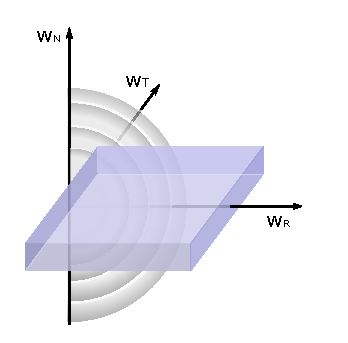
\includegraphics[width=.34\textwidth]{Figures/sketch_slice_N2.pdf}
	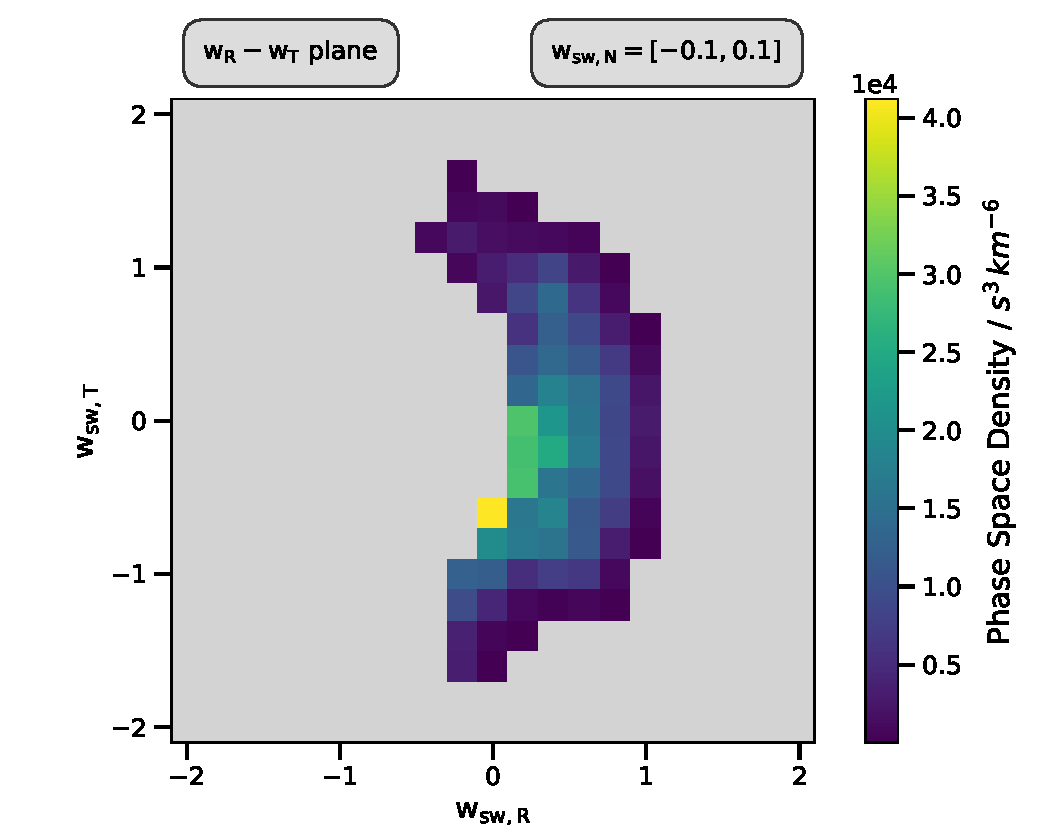
\includegraphics[width=.64\textwidth]{Figures/slice_50_N.pdf}
	\centering
	\caption{\textbf{Left:} Sketch of the orientation of a slice in the $w_R - w_T$ plane. A selection of ESA shells is shown in grey.\\ \textbf{Right:} Cartesian cut through the three-dimensional PSD for $\mathrm{He^{+}}$, measured during DOY 315-365 in 1993 for solar wind speeds from $760 \, \mathrm{km\,s^{-1}}$ to $780 \, \mathrm{km\,s^{-1}}$. The crescent shape results from SWICS' coverage.}
	\label{fig:sketch_slice_N}
\end{figure}
%
%
%
%
%
\clearpage
\noindent In Fig. \ref{fig:psd_lang} we show the PSD for another longer time period of 250 days in 1994 at solar wind speeds $740 \, \mathrm{km\,s^{-1}}$ to $780 \, \mathrm{km\,s^{-1}}$ for a slice $0.1 <= w_\mathrm{sw,R} < 0.3$. Corresponding Counts and PSV are shown in Fig. \ref{fig:counts_long} and \ref{fig:norm_long}. Here, the counts show a ring structure which vanishes by normalization. 
The PSD in  Fig. \ref{fig:psd_lang} shows distribution similar to the PSD from the shorter time period in 1993, concentrated and symmetrical around the central radial direction.
\begin{figure}[h]
	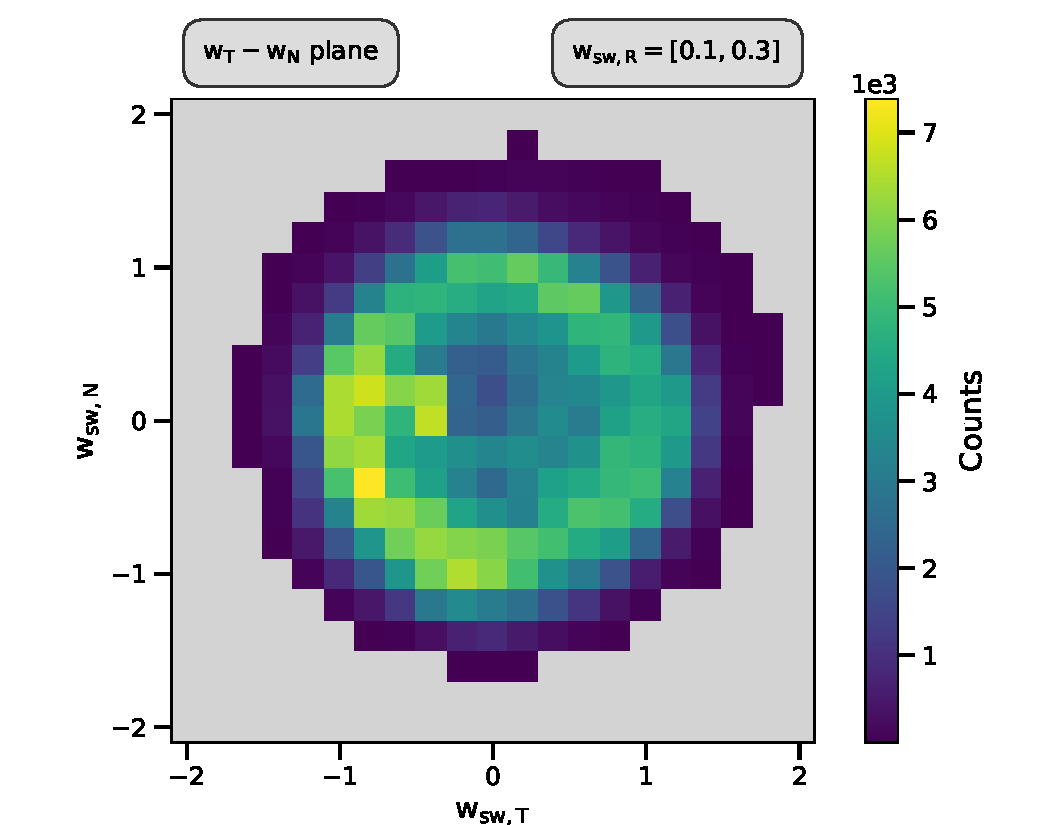
\includegraphics[width=.85\textwidth]{Figures/cart_long_counts.pdf}
	\centering
	\caption{Cartesian cut through $\mathrm{He^{+}}$ count distribution in a 3D $w_\mathrm{sw}$-space, measured during DOY 1-250 in 1994 for solar wind speeds from $740 \, \mathrm{km\,s^{-1}}$ to $780 \, \mathrm{km\,s^{-1}}$.}
	\label{fig:counts_long}
\end{figure}
\begin{figure}[h]
	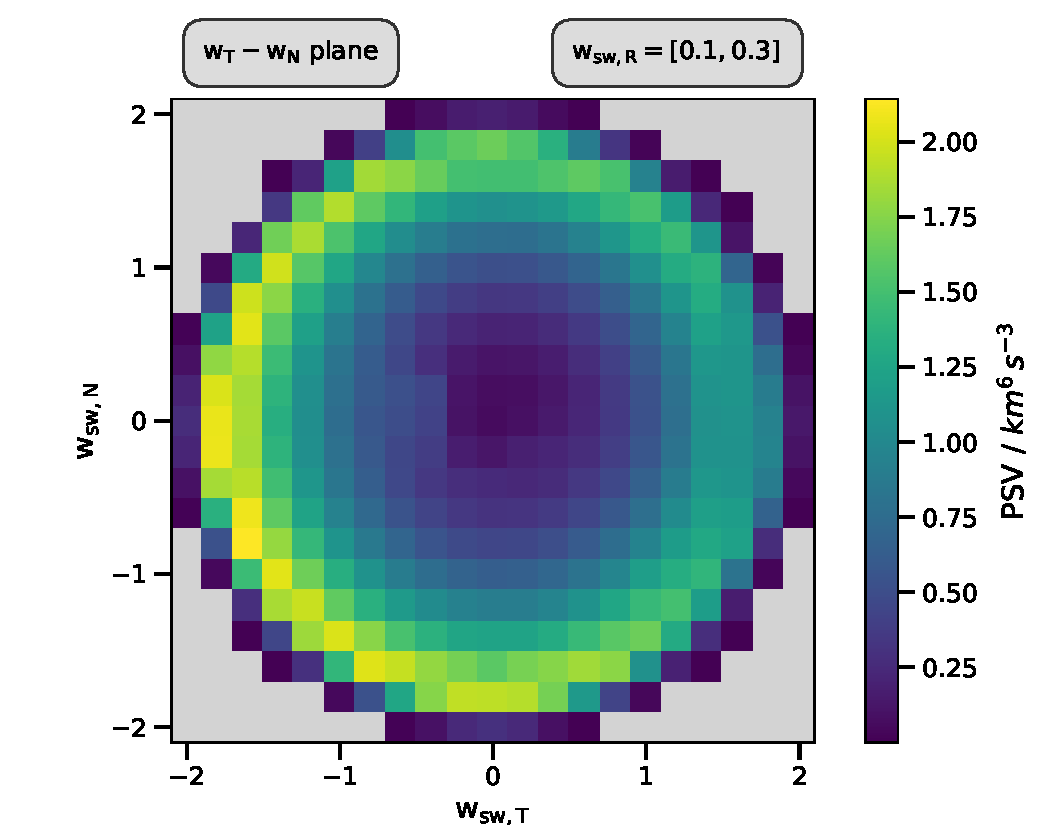
\includegraphics[width=.85\textwidth]{Figures/cart_long_norm.pdf}
	\centering
	\caption{Cartesian cut through the integrated observed PSV in a 3D $w\mathrm{sw}$-space, measured during DOY 1-250 in 1994 for solar wind speeds from $740 \, \mathrm{km\,s^{-1}}$ to $780 \, \mathrm{km\,s^{-1}}$.}
	\label{fig:norm_long}
\end{figure}
\begin{figure}[h]
	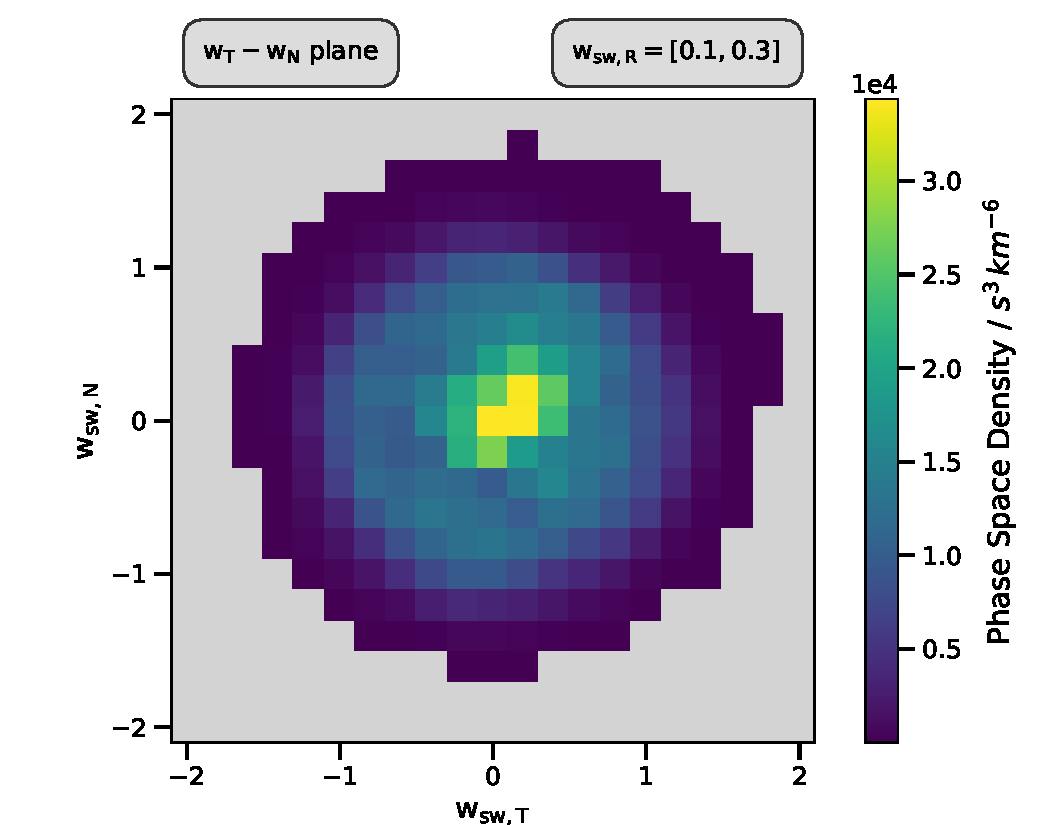
\includegraphics[width=.85\textwidth]{Figures/cart_long_ps.pdf}
	\centering
	\caption{Cartesian cut through the three-dimensional PSD for $\mathrm{He^{+}}$, measured during DOY 1-250 in 1994 for solar wind speeds from $740 \, \mathrm{km\,s^{-1}}$ to $780 \, \mathrm{km\,s^{-1}}$}
	\label{fig:psd_lang}
\end{figure}
%
%
%
%
%
\clearpage
\section{Spherical Projection}
Of course we are not limited to the presented Cartesian projections.
We can also choose a shell-wise projection. For this we consider spherical shells of constant $w\mathrm{sw}$ in the solar wind frame. For better understanding we can refer to Fig. \ref{fig:cov} again. Here we see the blue rings as 2D cuts through such concentric shells around $w\mathrm{sw} = 0$. The spherical coordinate $\varphi$ is measured within the $w_\mathrm{sw,T}-w_\mathrm{sw,N}$ plane with $\varphi = 0^\circ$ for $w_\mathrm{sw,T} = 0$ and $\varphi > 0^\circ$ for negative values $w_\mathrm{sw,T}$. The second coordinate $\vartheta$ is defined perpendicular to the $w_\mathrm{sw,T}-w_\mathrm{sw,N}$ plane. It is $\vartheta = 0 ^\circ$ for values within the plane and $\vartheta = 90^\circ$ along the positive $w_\mathrm{sw,N}$ axis (out of the paper plane).
\\
In Figs. \ref{fig:sky_counts} and \ref{fig:sky_norm} we show counts and integrated PSV in this projection for $\mathrm{He^{+}}$ measurements from 50 days in 1993, restricted to solar wind speeds from $760 \, \mathrm{km\,s^{-1}}$ to $780 \, \mathrm{km\,s^{-1}}$. The selected spherical shell comprises absolute $w$-values $0.85 <= w_\mathrm{sw} < 0.95$. Considering the definition of the two coordinates $\varphi$ and $\vartheta$ we find, that the central viewing direction against the $w_\mathrm{sw,R}$ axis in Fig. \ref{fig:cov}. Even more clearly than in the Cartesian projection sharp peaks around $\varphi = 30 ^\circ$ and $\vartheta = 0 ^\circ$ are apparent in both figures \ref{fig:sky_counts} and \ref{fig:sky_norm}, which is due to the variation in observation time of PSV. The histogram of the corresponding PSD, that excludes this effect, is shown in Fig. \ref{fig:sky_psd}.\\
This spherical projection can become particularly suitable for the examination of the level of isotropy within a $w_\mathrm{sw}$-shell. Shapes like a torus distribution (s. Sec. \ref{sec:theo_vdf}) can be observed directly. For a completely isotropized shell we would expect an evenly colored projection in Fig. \ref{fig:sky_psd}. This is obviously not the case. Here, we find a structure of increased PSD that is around $-60\,^\circ$ longitude for $\vartheta = 0\,^\circ$ and moves towards $\varphi = 0\,^\circ$ for higher latitudes.
\\
Unfortunately, we could not find clear structures that were constant over different periods of measurement. A possible reason for that could be that we could only very vaguely determine the detection efficiency in Sec. \ref{subsec:det_eff}. As the spherical projection comprises measurements from different ESA steps (s. \ref{fig:cov}), an inaccurate efficiency weighting could either lead to a disappearance of real structures or even to an emerging of artificial ones. A detailed analysis of the detection efficiencies as it is shown in \citet{koeten} for ACE/SWICS is beyond the scope of this work but would be highly beneficial for future analyses.
\begin{figure}[h]
	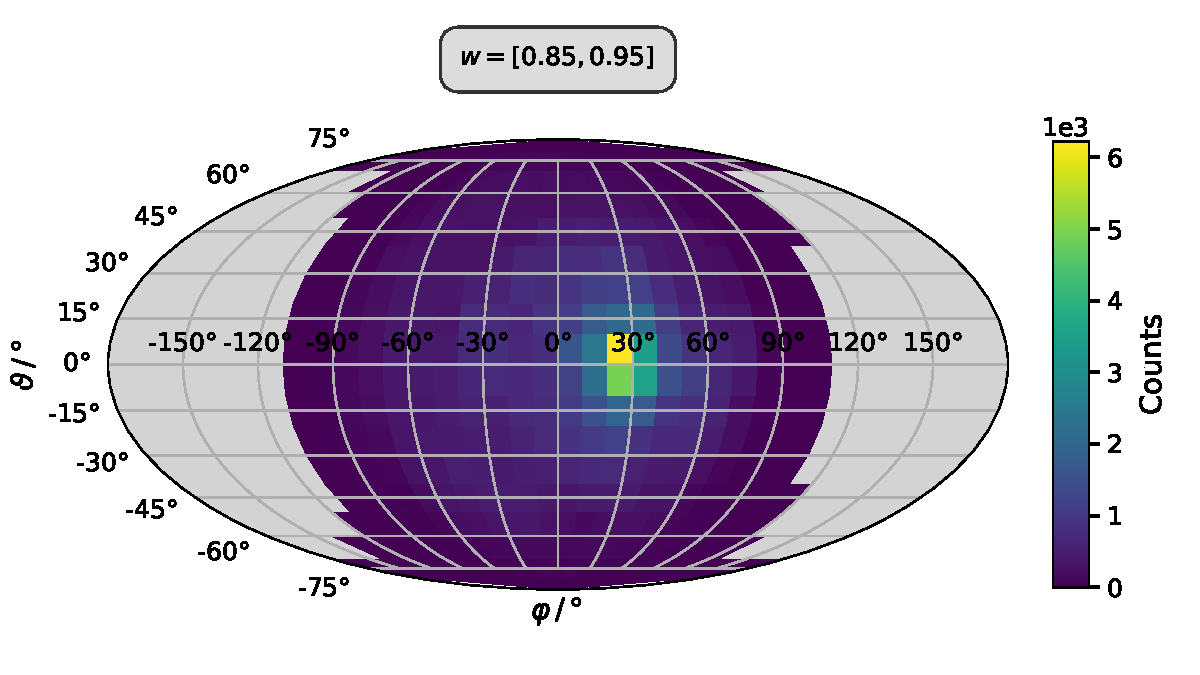
\includegraphics[width=1\textwidth]{Figures/sky_counts.pdf}
	\centering
	\caption{Spherical projection of $\mathrm{He^{+}}$ count distribution in a 3D $w_\mathrm{sw}$-space, measured during DOY 315-365 in 1993 for solar wind speeds from $760 \, \mathrm{km\,s^{-1}}$ to $780 \, \mathrm{km\,s^{-1}}$. Grey areas depict PSV that has not been observed and result from SWICS' coverage.}
	\label{fig:sky_counts}
\end{figure}
\begin{figure}[h]
	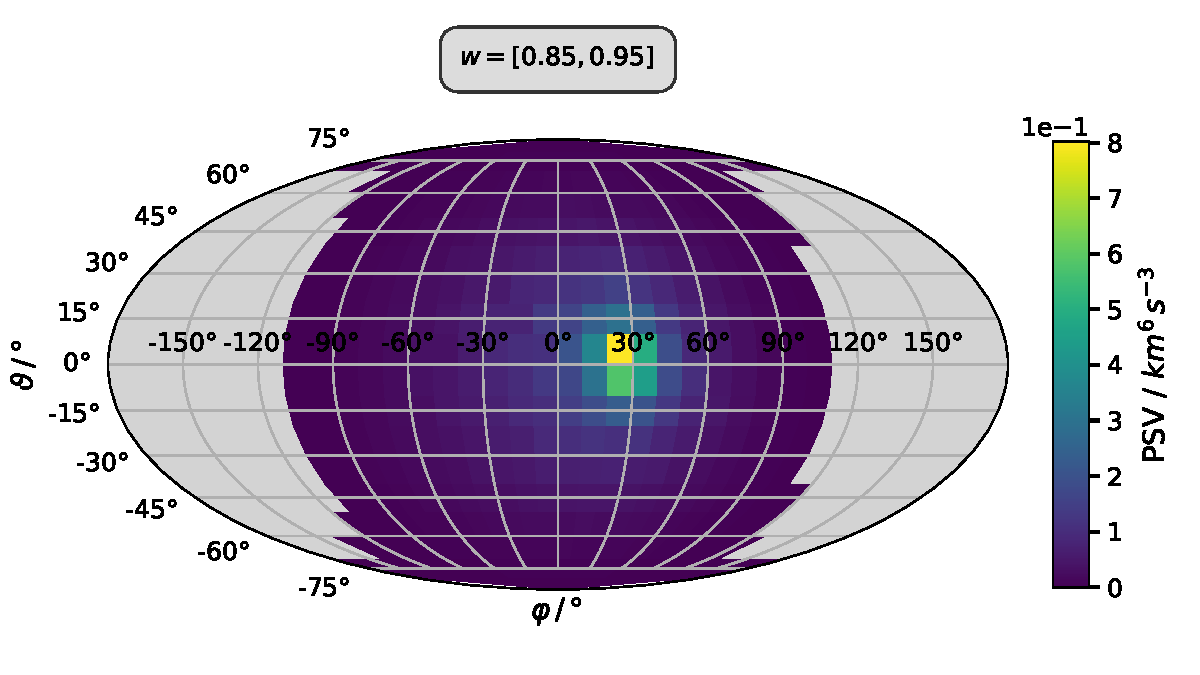
\includegraphics[width=1\textwidth]{Figures/sky_norm.pdf}
	\centering
	\caption{Spherical projection of the integrated observed PSV in a 3D $w_\mathrm{sw}$-space, measured during DOY 315-365 in 1993 for solar wind speeds from $760 \, \mathrm{km\,s^{-1}}$ to $780 \, \mathrm{km\,s^{-1}}$. Grey areas depict PSV that has not been observed and result from SWICS' coverage.}
	\label{fig:sky_norm}
\end{figure}
\begin{figure}[h]
	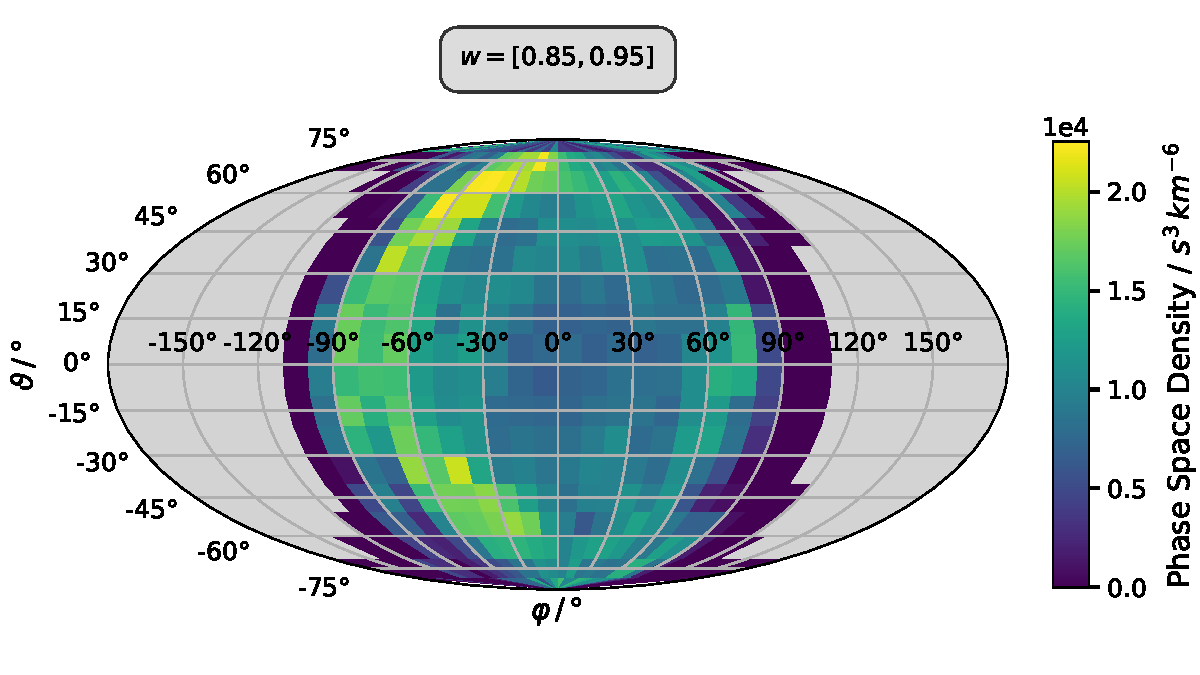
\includegraphics[width=1\textwidth]{Figures/sky_ps.pdf}
	\centering
	\caption{Spherical projection of the three-dimensional PSD for $\mathrm{He^{+}}$, measured during DOY 315-365 in 1993 for solar wind speeds from $760 \, \mathrm{km\,s^{-1}}$ to $780 \, \mathrm{km\,s^{-1}}$. Grey areas depict PSV that has not been observed and result from SWICS' coverage.}
	\label{fig:sky_psd}
\end{figure}
%
%
%
\clearpage
\section{1D Projection}
In this last section we show 1D projections of three-dimensional velocity distributions from measurements of two different years. In each year (1994, 1996) we analyzed $\mathrm{He^{+}}$ data from 100 days at solar wind speeds from $760 \, \mathrm{km\,s^{-1}}$ to $770 \, \mathrm{km\,s^{-1}}$.\\
For this projection we integrate both the counts and the PSV over spherical shells around $w_\mathrm{sw}=0$. In a 2D cut this can be visualized by an integration along a blue circle in Fig. \ref{fig:cov}. We combined values within the width $\Delta w_\mathrm{sw} = 0.1$ at different radii from $w_\mathrm{sw} = 0.25$ to $w_\mathrm{sw} = 1.05$. In Fig. \ref{fig:1d} the histogram of the resulting PSD is shown. The histograms look qualitatively similar for both years. 
We see a relatively broad distribution with a clear cutoff around $w = 1$, which corresponds to $w_\mathrm{sc} = 2$ (s. Sec. \ref{sec:theo_vdf}, Ch. \ref{chap:intro}). For smaller values of $w_\mathrm{sw}$ the distribution does not change over many magnitudes. 
\\
The spectra in Fig. \ref{fig:1d} are also in good qualitative agreement with the one in Fig. \ref{fig:gloeckler}. It should be noted that our spectra are limited to values $w_\mathrm{sw} > 0.25$, while the spectrum in Fig. \ref{fig:gloeckler} is continued down to values $w_\mathrm{sc} < 1$, which corresponds to values $w_\mathrm{sw} < 0$ in solar wind frame. In Sec. \ref{subsec:cov} we have seen that $\mathrm{He^{+}}$ Triple Coincidences can only be measured for distinct $w$-values above a limit that is dependent on the solar wind speed but hardly smaller than $w_\mathrm{sw} = 1$. This shows that the spectrum in Fig. \ref{fig:gloeckler} is not based on solely Triple Coincidences but also on $\mathrm{He^{+}}$ Double Coincidences. As Double Coincidences lack an energy measurement in the solid-state detector and thus a directional resolution, the spectrum can only result from an integration along different ESA shells that is projected onto a distinct possible value.
Although the spectra look similar we want to emphasize that the spectrum in Fig. \ref{fig:1d} results from a very different approach as we show projected cuts through an actual three-dimensional velocity distribution.
\begin{figure}[h]
	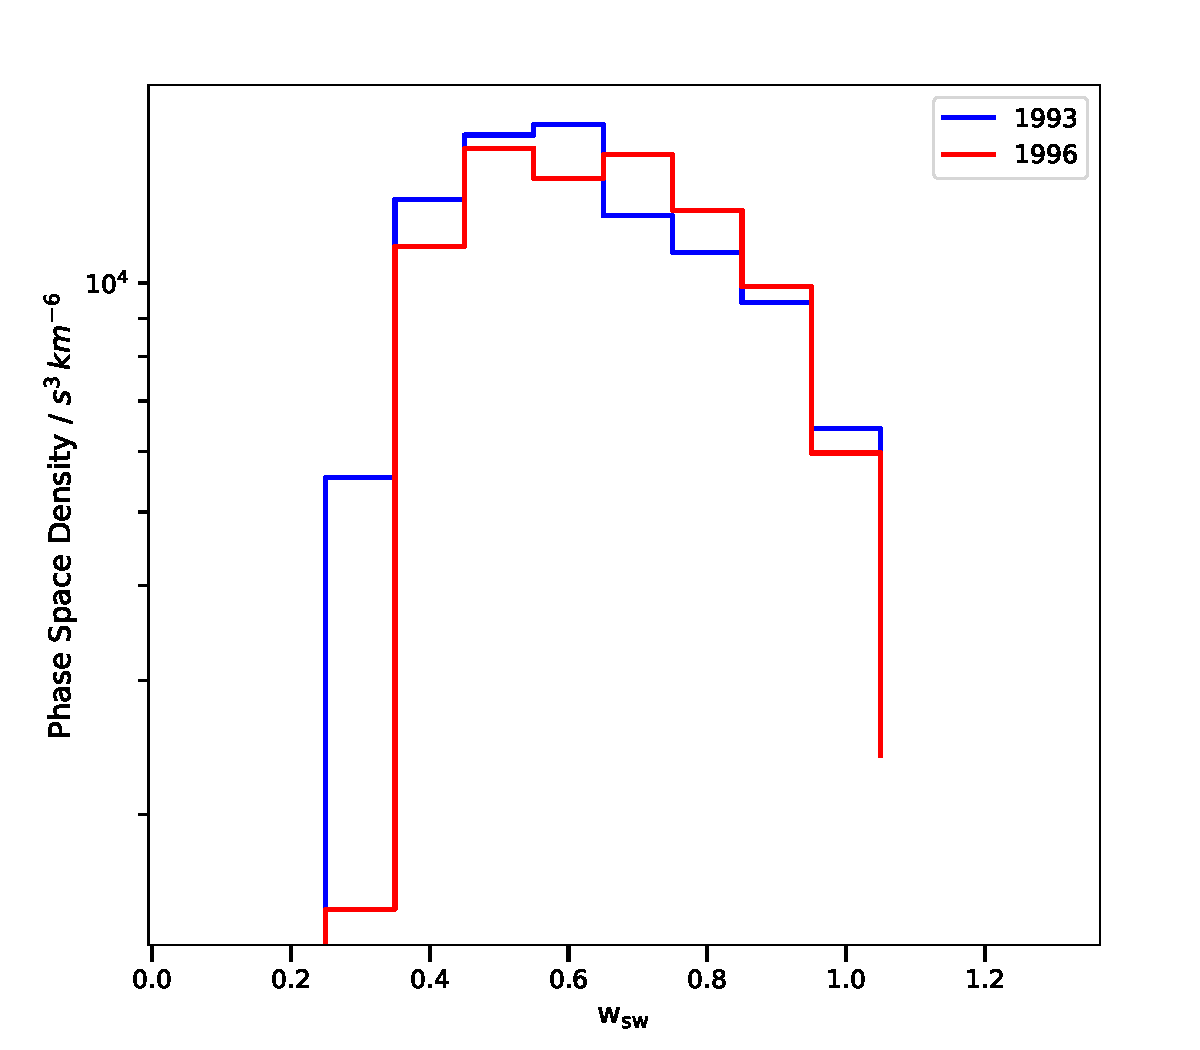
\includegraphics[width=.8\textwidth]{Figures/1D.pdf}
	\centering
	\caption{1D projected PSD from a 3D $w_\mathrm{sw}$-space, measured during DOY 1-100 in 1994 and 1996 for solar wind speeds from $760 \, \mathrm{km\,s^{-1}}$ to $770 \, \mathrm{km\,s^{-1}}$}
	\label{fig:1d}
\end{figure}